\documentclass[11pt, oneside]{article} 
\usepackage{geometry}
\geometry{letterpaper} 
\usepackage{graphicx}
	
\usepackage{amssymb}
\usepackage{amsmath}
\usepackage{parskip}
\usepackage{color}
\usepackage{hyperref}

\graphicspath{{/Users/telliott_admin/Tex/png/}}
% \begin{center} 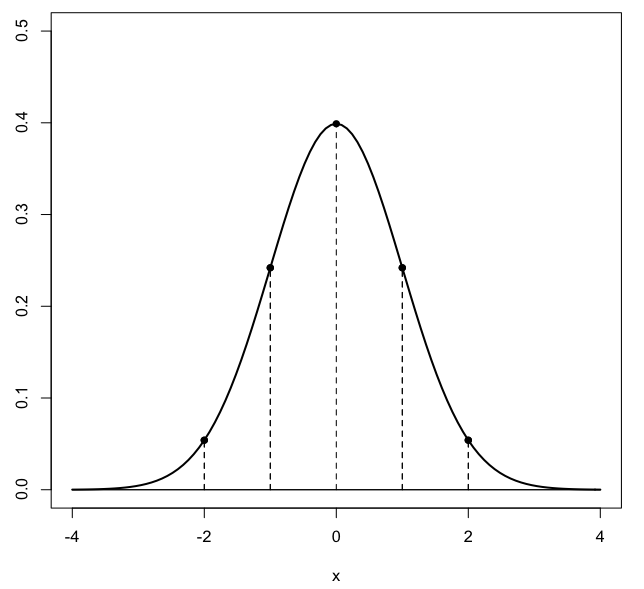
\includegraphics [scale=0.4] {gauss3.png} \end{center}

\title{Dipole in a field}
\date{}

\begin{document}
\maketitle
\Large

Consider a dipole with a total separation $2a$ between the charges, $+q$ and $-q$.  The dipole lies in a uniform electric field $E$ (say it is horizontal) at an angle to the field lines of $\theta$.

\begin{center} 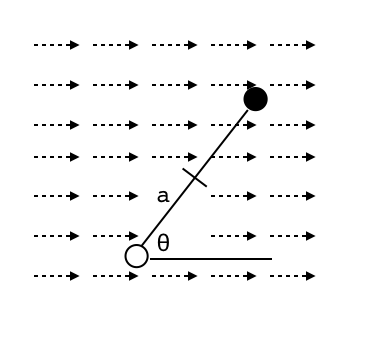
\includegraphics [scale=0.4] {dipole_field.png} \end{center}

The forces on the two charges from the field cancel.  

However, there are also two torques, which both tend to align the dipole with the field.  For the charge $+q$, there is a force $Eq$.  The torque is that component of the force perpendicular to the axis of the dipole, $F \sin \theta$, times the distance from the axis of rotation at the point where the force is applied, which is equal to $a$.

\[ \tau = aEq \sin \theta \]
Since there are two charges, the torque is double:
\[ \tau = 2aEq \sin \theta \]
Even though the second charge is negative, the force on it tends to rotate the dipole in the same direction as the force on the positive charge.

$2aq$ is equal to the dipole moment, $p$ so
\[ \tau = pE \sin \theta \]
but this is
\[ \tau = \mathbf{p} \times \mathbf{E}  \]

The order of the two terms in the cross-product is a matter of definition:  $\tau = \mathbf{r} \times \mathbf{F}$.  This order makes the resulting vector point into the page.

There is a potential energy when the dipole lies at an angle to the field.  For work done by a force we would write
\[ U = -W = \int \mathbf{F} \cdot d \mathbf{r} \]
The equivalent formulation for torque is
\[ \int \mathbf{\tau} \cdot d \theta = \int_{\theta_0}^{\theta} pE \sin \theta \]
\[ = -pE \cos \theta \ \bigg |_{\theta_0}^{\theta} \]

If we choose $\theta_0$ corresponding to zero potential energy

\[ U = pE \cos \theta = \mathbf{p} \cdot \mathbf{E} \]

When $\theta$ is 90 degrees and the dipole is perpendicular to the field, the potential energy is $pE$.

\end{document}